\documentclass{standalone}
\usepackage[T1]{fontenc}
\usepackage[utf8]{inputenc}
\usepackage{pgf,tikz}
\usepackage{setspace}
\usepackage{pgfplots}
\pgfplotsset{compat=1.13}
\usepackage{romannum}

\usepgfplotslibrary{groupplots}

\begin{document}


\def\TT{1.0}

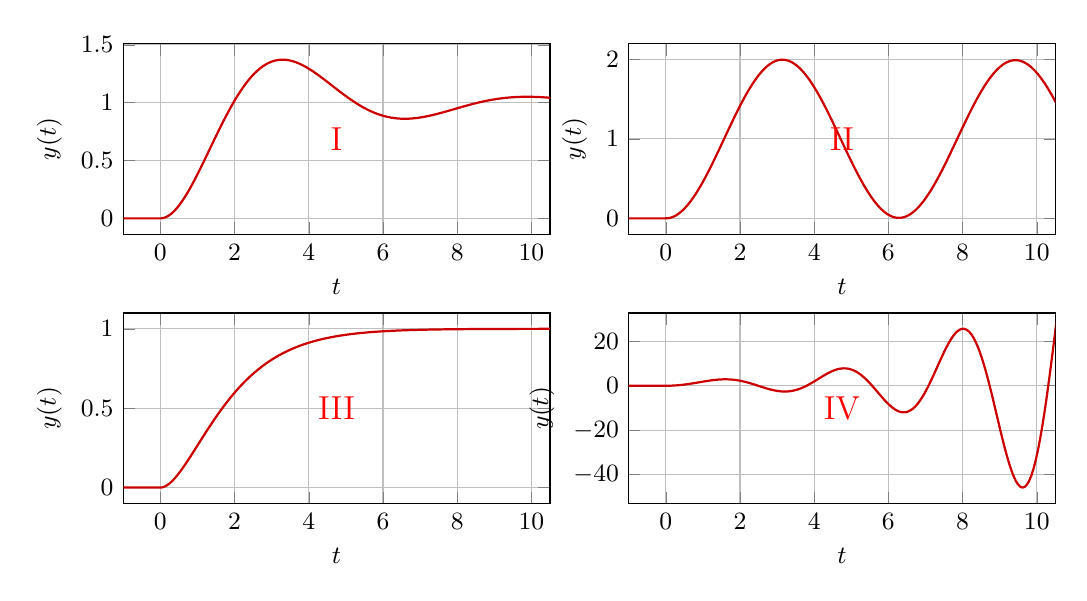
\begin{tikzpicture}

  
  \pgfmathsetmacro{\wwone}{1}
  \pgfmathsetmacro{\zzone}{0.3}
  \pgfmathsetmacro{\wwtwo}{1}
  \pgfmathsetmacro{\zztwo}{0.001}
  \pgfmathsetmacro{\wwthree}{1}
  \pgfmathsetmacro{\zzthree}{0.99}
  \pgfmathsetmacro{\wwfour}{2}
  \pgfmathsetmacro{\zzfour}{-0.2}

  \begin{groupplot}[
  group style={group size=2 by 2},height=4cm,width=7cm,
  /tikz/font=\small,
  %xtick=0,
  %ytick=\empty,
  xlabel={$t$}, 
  ylabel={$y(t)$},
  xmin=-1,
  xmax=10.5,
  grid = both,
  ]

  
  \nextgroupplot
  \addplot+[thick, red!80!black, no marks, domain=-1:11, samples=200] {(x>0)*(1-exp(-x*\wwone*\zzone)/sqrt(1 - \zzone*\zzone) * sin(x*180/3.1415*(\wwone*sqrt(1 - \zzone*\zzone)) + acos(\zzone)))};
  
  
    \nextgroupplot
    \addplot+[thick, red!80!black, no marks, domain=-1:11, samples=200] {(x>0)*(1-exp(-x*\wwtwo*\zztwo)/sqrt(1 - \zztwo*\zztwo) * sin(x*180/3.1415*(\wwtwo*sqrt(1 - \zztwo*\zztwo)) + acos(\zztwo)))};

  
    \nextgroupplot
    \addplot+[thick, red!80!black, no marks, domain=-1:11, samples=200] {(x>0)*(1-exp(-x*\wwthree*\zzthree)/sqrt(1 - \zzthree*\zzthree) * sin(x*180/3.1415*(\wwthree*sqrt(1 - \zzthree*\zzthree)) + acos(\zzthree)))};

    \nextgroupplot
    \addplot+[thick, red!80!black, no marks, domain=-1:11, samples=200] {(x>0)*(1-exp(-x*\wwfour*\zzfour)/sqrt(1 - \zzfour*\zzfour) * sin(x*180/3.1415*(\wwfour*sqrt(1 - \zzfour*\zzfour)) + acos(\zzfour)))};

  \end{groupplot}

  \node[red] at (group c1r1.center) {\large \Romannum{1}};
  \node[red] at (group c2r1.center) {\large \Romannum{2}};
  \node[red] at (group c1r2.center) {\large \Romannum{3}};
  \node[red] at (group c2r2.center) {\large \Romannum{4}};

\end{tikzpicture}
\end{document}

